% begin module limit-at-infinity-ex4
\begin{frame}
\begin{example}
Find the horizontal and vertical asymptotes of $f(x) = \frac{\sqrt{3x^2+1}}{2x-3}$.
\begin{columns}[c]
\column{.35\textwidth}
\psset{xunit=0.45cm, yunit=0.45cm}
\begin{pspicture}(-5, -5)(5.1,5.1)
\psframe*[linecolor=white](-5,-5)(5.1,5.1)
\psaxes[ticks=none, labels=none]{<->}(0,0)(-5,-5)(5,5)\tiny
\fcLabels{5}{5}

\only<handout:1| 25->{ %
%Function formula: ((1+2 ((x)^{2}))^{1/2})/(-5+3 (x))
\psplot[linecolor=red, plotpoints=1000]{3 2 div 0.335 add}{5}{x x mul 3 mul 1 add sqrt 2 x mul 3 sub div }
\psplot[linecolor=red, plotpoints=1000]{-5}{3 2 div 0.245 sub}{x x mul 3 mul 1 add sqrt 2 x mul 3 sub div}
\rput[l](3,3){$y=f(x)$}
}

\only<handout:1| 24->{ %
\psline[linecolor=blue, linestyle=dashed](! 3 2 div -4.95)(! 3 2 div 4.95)
\rput[l](1.7, -2.5){$x=\frac{3}{2}$}
}

\only<handout:1| 18->{ %
\psline[linecolor=blue, linestyle=dashed](! -4.95 3 sqrt 2 div)(! 4.95 3 sqrt 2 div)
\rput[b](-3, 0.89){$\frac{\sqrt{3}}{2}$}
}
\only<handout:1| 22->{ %
\psline[linecolor=blue, linestyle=dashed](! -4.95 3 sqrt -2 div)(! 4.95 3 sqrt -2 div)
\rput[t](-3, -0.89){$-\frac{\sqrt{3}}{2}$}
}
\end{pspicture}
%\ \only<handout:0| -17>{%
%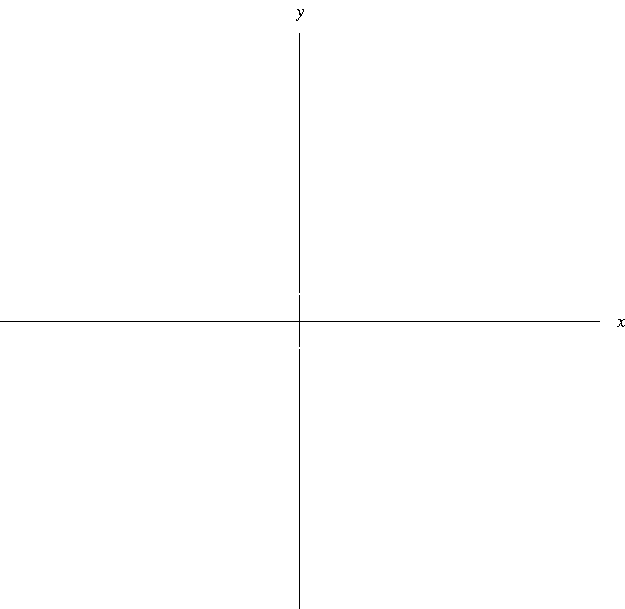
\includegraphics[width=4.5cm]{curve-sketching/pictures/04-04-ex4a.pdf}%
%}%
%\only<handout:0| 18-21>{%
%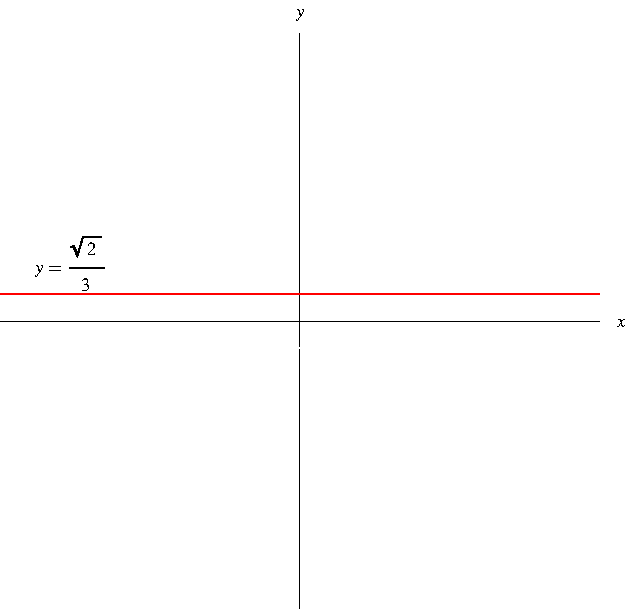
\includegraphics[width=4.5cm]{curve-sketching/pictures/04-04-ex4b.pdf}%
%}%
%\only<handout:0| 22-23>{%
%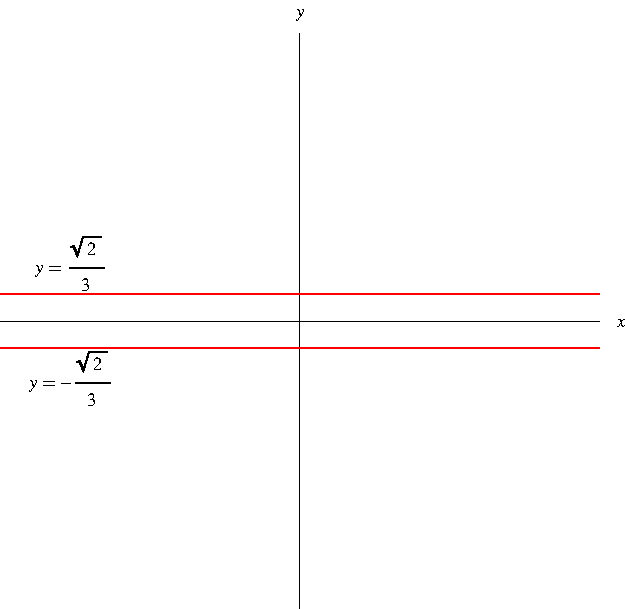
\includegraphics[width=4.5cm]{curve-sketching/pictures/04-04-ex4c.pdf}%
%}%
%\only<handout:0| 24>{%
%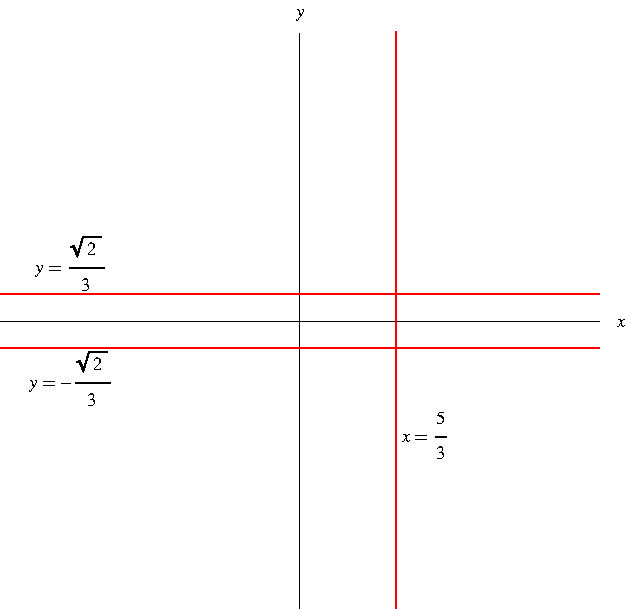
\includegraphics[width=4.5cm]{curve-sketching/pictures/04-04-ex4d.pdf}%
%}%
%\only<25->{%
%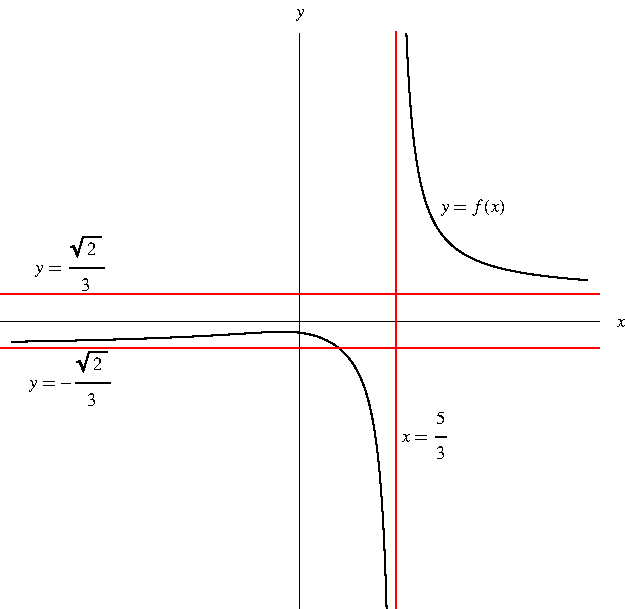
\includegraphics[width=4.5cm]{curve-sketching/pictures/04-04-ex4e.pdf}%
%}%
%\begin{itemize}

\uncover<4->{\alertNoH{ 4}{If $x > 0$ then $x = \sqrt{x^2}$.}}

\uncover<20->{\alertNoH{ 20}{If $x < 0$ then $x = -\sqrt{x^2}$.}}

\uncover<23->{\alertNoH{ 23-24}{Vertical Asymptote: \uncover<24-25>{$x = \frac{3}{2}$.}}}
%\end{itemize}
\column{.65\textwidth}

\abovedisplayskip=0pt
\belowdisplayskip=0pt
\[
\begin{array}{l}
\uncover<2->{%
\displaystyle \lim_{x\to \infty} \frac{\sqrt{3x^2+1}}{2\alertNoH{ 3}{x}-3}\uncover<3->{\alertNoH{ 3}{\cdot \frac{\alertNoH{ 4}{\frac{1}{x}}}{\frac{1}{x}}}}%
}%
%\\%
%& \uncover<4->{ = } &%
\uncover<4->{%
\displaystyle = \lim_{x\to \infty} \frac{\alertNoH{ 5-6}{\sqrt{3x^2+1}}}{\alertNoH{ 7-8}{2x-3}}\cdot \frac{\alertNoH{ 4-6}{ \frac{1}{ \sqrt{x^2}} }}{\alertNoH{ 7-8}{\frac{1}{x}}}%
}%
\\%
%& \uncover<8->{ = } &%
\uncover<5->{%
\displaystyle = \lim_{x\to \infty} \frac{\alertNoH{ 5-6}{\sqrt{ \fcAnswer{6}{3+\frac{1}{x^2}}}}}{\fcAnswerUncover{5}{8}{2- \frac{3}{x}} }%
}%
\uncover<9->{%
\displaystyle = \frac{\sqrt{\displaystyle \alertNoH{ 10-11}{ \lim_{x\to\infty}3} + \alertNoH{ 12-13}{ \lim_{x\to\infty}\frac{1}{x^2}}}}{\displaystyle \alertNoH{ 14-15}{\lim_{x\to\infty}2} - \alertNoH{ 16-17}{3 \lim_{x\to\infty}\frac{1}{x}}}%
}%
\\%
%& \uncover<9->{ = } &%
\uncover<10->{%
\displaystyle = \frac{\sqrt{\fcAnswerUncover{10}{ 11}{3} + \fcAnswerUncover{10}{ 13}{0} }  }{ \fcAnswerUncover{10}{ 15}{2} - \fcAnswerUncover{10}{ 17}{0}}%
}%
\uncover<18->{%
 = \frac{\sqrt{3}}{2}%
}%
\end{array}
\]

\abovedisplayskip=0pt
\belowdisplayskip=0pt
\[
\begin{array}{l}
\uncover<2->{%
\displaystyle \lim_{x\to -\infty} \frac{\sqrt{3x^2+1}}{2 \alertNoH{ 19}{x}-3 }\uncover<19->{\alertNoH{ 19}{\cdot \frac{\alertNoH{ 20}{ \frac{1}{ x}} }{\frac{1}{x}}}}%
}%
\uncover<20->{%
\displaystyle = \lim_{x\to -\infty} \frac{\sqrt{3x^2 +1}}{ 2x- 3}\cdot \frac{\alertNoH{ 20}{\frac{-1}{\sqrt{x^2}}}}{\frac{1}{x}}%
}%
\\%
\uncover<21->{%
\displaystyle = \lim_{x\to -\infty} -\frac{\sqrt{3+\frac{1 }{x^2}}}{2 -\frac{3}{x}}%
}%
\uncover<22->{%
\displaystyle = -\frac{\sqrt{3}}{2}
}%
\end{array}
\]

\end{columns}
\end{example}
\end{frame}
% end module limit-at-infinity-ex4
